\documentclass[a4paper,11pt,oneside]{article}

\usepackage{amsmath,amssymb,epsfig}
\usepackage[T1]{fontenc}
\usepackage{ae,aecompl}
\usepackage{url}
\usepackage{subfigure}
\addtolength{\voffset}{-.5cm}
\addtolength{\hoffset}{-.5cm}
\setlength{\parindent}{0in}
\addtolength{\textwidth}{.5cm}
\addtolength{\textheight}{.51cm}
\addtolength{\parskip}{.5cm}

% Example definitions.
% --------------------
\def\e{{e^{j\omega}}}
\def\W{{W_M}}
\def\sumk{{\sum_{k=-\infty}^{\infty}}}
\def\x{{\mathbf x}}
\def\X{{\mathbf X}}
\def\Y{{\mathbf Y}}
\def\u{{\mathbf u}}
\def\U{{\mathbf U}}
\def\x{{\mathbf x}}
\def\s{{\mathbf s}}
\def\A{{\mathbf A}}
\def\y{{\mathbf y}}
\def\w{{\mathbf w}}
\def\B{{\mathbf B}}
\def\a{{\mathbf a}}
\def\D{{\mathbf D}}
\def\P{{\mathbf P}}
\def\n{{\mathbf n}}
\def\V{{\mathbf V}}
\def\R{{\mathbf R}}
\def\I{{\mathbf I}}
\def\M{{\mathbf M}}
\def\sech{{\mathrm{sech}}}
\def\L{{\cal L}}
\def\Cum{{\rm{Cum}}}
\def\var{{\rm{var}}}
\def\T{{\mathbf T}}
\def\C{{\mathbf C}}
\def\tf{{\emph{t-f}}}


% Title.
% ------
\title{SGN-1107 Introductory Signal Processing\\
Sample exam}
%
% Author and date.
% ---------------
\date{\today}
\author{Germ\'an G\'omez-Herrero, \url{http://germangh.com}}



\begin{document}
\maketitle



\textbf{QUESTION 1 (5 points):} An L-th order moving average filter is a system that, for an input $x[n]$ produces the output:
\[
y[n] = \frac{1}{1+L}\sum_{k=0}^{L}x[n-k]
\]
Is this system linear? Is it time-invariant? Justify your answers. Find the system's impulse response $h[n]$ and frequency response $H(e^{j\omega})$.

\vspace{1cm}

\textbf{SOLUTION:}

\textbf{Is the system linear?}

Consider the input sequence $a[n]=\alpha x_1[n]+\beta x_2[n]$ with $\alpha$ and $\beta$ being two arbitrary scalar and $x_1[n]$ and $x_[n]$ being two arbitrary sequences. Then, if the system is linear, it must be satisfy that the output to $x[n]$ is $y_a[n]=\alpha y_1[n] + \beta y_2[n]$ where $y_1[n]$ and $y_2[n]$ are the outputs of the system to the inputs $x_1[n]$ and $x_2[n]$, respectively. We can easily check that:

\[
\begin{array}{lll}
y_a[n] &=& \frac{1}{1+L}\sum_{k=0}^{L}a[n-k]=\frac{1}{1+L}\sum_{k=0}^{L} \left(\alpha x_1[n-k]+\beta x_2[n-k]\right)\\
&=&\alpha\left(\frac{1}{1+L}\sum_{k=0}^{L}x_1[n-k]\right)+\beta\left(\frac{1}{1+L}\sum_{k=0}^{L}x_2[n-k]\right)\\
&=&\alpha y_1[n] + \beta y_2[n]
\end{array}
\]

So the system is linear.

\textbf{Is the system time-invariant?}

The system will be time invariant if a delayed input $x[n-\tau]$ produces a delayed output $y[n-\tau]$. Let us denote by $y_\tau[n]$ the output produced by $x[n-\tau]$. Then we can easily check that:

\[
y_\tau[n] = \frac{1}{1+L}\sum_{k=0}^{L}x[n-k-\tau]=y[n-\tau]
\]

so the system is time-invariant.

\textbf{Impulse response and frequency response}

The impulse response can be obtained directly from the input-output relationship by using as input sequence a unitary impulse, that is $x[n]=\delta[n]$. Then, the impulse response is:

\[
h[n] = \frac{1}{1+L}\sum_{k=0}^{L}\delta[n-k]
\]

And the frequency response can be obtained using the discrete-time Fourier transform (DTFT):

\[
H(e^{j\omega})=\sum_{n=-\infty}^{\infty}h[n]e^{-j\omega n}=\frac{1}{1+L}\sum_{k=0}^{L}e^{-j\omega k}\\
=\frac{1}{L+1}\cdot \frac{e^{j\omega}-e^{-j\omega L}}{e^{j\omega -1}}
\]


\vspace{1cm}

\textbf{QUESTION 2 (5 points):} Consider the system defined by the difference equation 

\[
y[n] = ay[n-1]+bx[n]+x[n-1]
\]

where $a$ and $b$ are real, and $|a|<1$.
\begin{itemize}
\item[(a)] Find the relationship between $a$ and $b$ that must exist if the frequency response is to have a constant magnitude for all $\omega$, that is $|H(e^{j\omega})|=1$.
\item[(b)] Assuming that this relationship is satisfied, find the output $y[n]$ of the system when $a=\frac{1}{2}$ and $x[n]=\left(\frac{1}{2}\right)^n\mu[n]$.
\end{itemize}

\vspace{1cm}

\textbf{SOLUTION:} 


\textbf{(a)}

In order to obtain the frequency response of the system, first we need to transform the system's equation into the frequency domain:

\[
Y(e^{j\omega})=ae^{-j\omega}Y(e^{j\omega})+bX(e^{j\omega})+e^{-j\omega}X(e^{j\omega})
\]

so the frequency response of the system is:

\[
H(e^{j\omega})=\frac{Y(e^{j\omega})}{X(e^{j\omega})}=\frac{b+e^{-j\omega}}{1-a\cdot e^{-j\omega}}
\]

If the equality $|H(e^{j\omega})|=1$ hold then it must also hold the equality $|H(e^{j\omega})|^2=1$. Solving this latter equality is easier because the expression on the left side has only real terms inside the absolute value operator. Operating a bit:

\[
|H(e^{j\omega})|^2=1 \Longrightarrow H(e^{j\omega})\cdot H^*(e^{j\omega})=1
\]

substituting the value of $H(e^{j\omega})$ into the expression above we obtain:

\[
H(e^{j\omega})\cdot H^*(e^{j\omega})=\frac{(b+e^{-j\omega})\cdot (b+e^{j\omega})}{(1-a\cdot e^{-j\omega})\cdot(1-a\cdot e^{j\omega})}=\frac{1+b^2+b\cdot(e^{j\omega}+e^{-j\omega})}{1+a^2-a\cdot(e^{j\omega}+e^{-j\omega})}=1
\]

So, the numerator and denominator of the fraction above must be equal, which translates into the two equations:

\[
\begin{array}{lll}
1+b^2&=&1+a^2\\
b &=& -a
\end{array}
\]

Clearly, if and only if $b=-a$ the two equations are fullfiled and $|H(e^{j\omega})|^2=1$. Since we have only a single solution to the squared version of our original condition we can conclude that this solution has to be also the solution to our original constraint. That is $|H(e^{j\omega})|=1$ if and only if $b=-a$.

\textbf{(b)}

If $a=\frac{1}{2}$ then the relationship that we found in $(a)$ tells us that $b=-a=-\frac{1}{2}$. We use the Z-transform to obtain the output of the system:

\[
x[n] = \left(\frac{1}{2}\right)^n\mu[n] \Longrightarrow X(z)=\frac{1}{1-\frac{1}{2}z^{-1}} \qquad \textrm{ROC}\equiv |z|>\frac{1}{2} 
\]

\[
H(e^{j\omega})=\frac{-\frac{1}{2}+e^{-j\omega}}{1-\frac{1}{2}\cdot e^{-j\omega}}\Longrightarrow H(z)=\frac{-\frac{1}{2}+z^{-1}}{1-\frac{1}{2}\cdot z^{-1}} \qquad \textrm{ROC}\equiv |z|>\frac{1}{2}
\]

\[
Y(z)=X(z)H(z)=-\frac{\frac{1}{2}z^{-1}}{(1-\frac{1}{2}z^{-1})^2}+2\frac{\frac{1}{2}z^{-1}}{(1-\frac{1}{2}z^{-1})^2}
\]

$Y(z)$ is directly invertible using the table of elementary pairs of Z-transforms. So, we finally obtain:

\[
y[n]=-(n+1)\left(\frac{1}{2}\right)^{n+1}\mu[n+1]+2n\left(\frac{1}{2}\right)^n\mu[n]
\]




\vspace{1cm}

\textbf{QUESTION 3 (5 points):} Diagrammed below is a hybrid digital-analog system. 
\begin{figure}[h!]
\centering
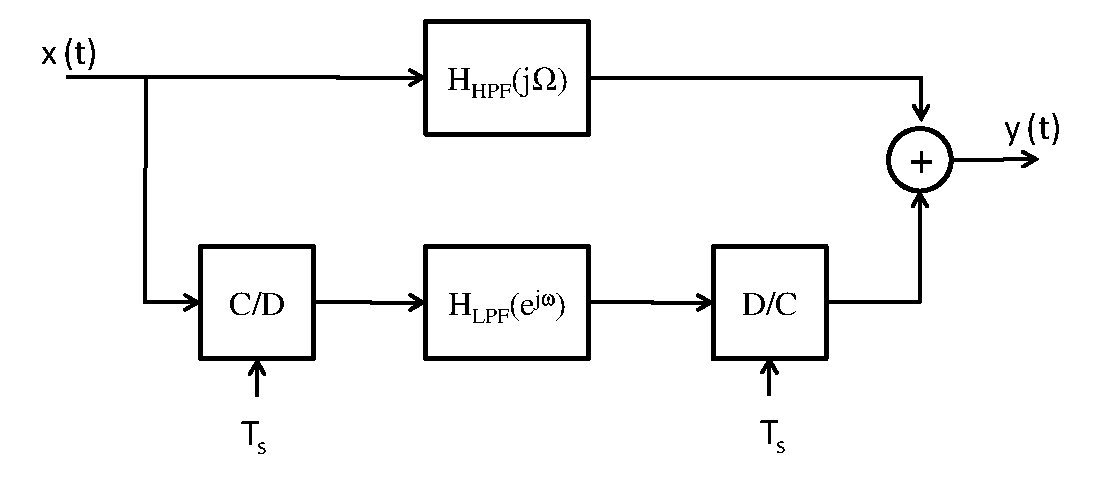
\includegraphics[width=.8\textwidth]{fig31.eps}
%\caption{Hybrid digital-analog system.}
\label{fig:fig2}
\end{figure}

The discrete-time system $H_{LPF}(e^{j\omega})$ is a low-pass filter:
\[
H_{LPF}(e^{j\omega})=\left\{\begin{array}{lll}
A & \qquad &|\omega|\leq \omega_{0}\\
0 & \qquad &\textrm{otherwise}
\end{array}\right.
\]
and the analog system is a filter with a frequency response as shown below: 

\begin{figure}[h!]
\centering
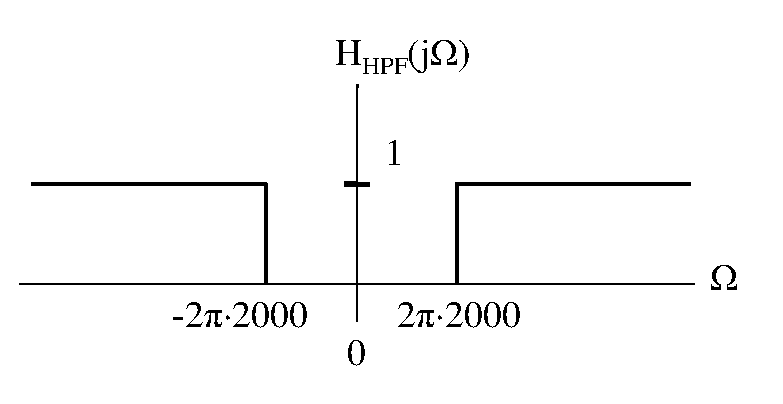
\includegraphics[width=.6\textwidth]{fig32.eps}
%\caption{Hybrid digital-analog system.}
\label{fig:fig3}
\end{figure}

The input analog signal is bandlimited to $\Omega_{0}=2\pi\cdot 4000$, and the sampling period of the ideal C/D and D/C converters is $T_s=10^{-4}$ seconds. Find values for A and $\omega_{0}$ that will result in perfect reconstruction of $x(t)$, i.e. values for which $y(t)=x(t)$.






\vspace{1cm}

\textbf{SOLUTION:} 

\emph{See solution of problem 4 from exercise session 3 for another view to this problem.}

First of all we have to check whether the sampling frequency is high enough so that aliasing in the discrete branch of the system is not going to prevent perfect reconstruction. The maximum analog frequency of the input signal that needs to be perfectly recovered is $\Omega_{max}=4000\cdot 2\pi$. Thus:

\[
T_{\textrm{Nyquist}}=T_{max}=\frac{2\pi}{2\Omega_{max}}=\frac{1}{8}\cdot 10^{-3}\; \textrm{seconds}
\]

So the maximum sampling period that is allowed to avoid aliasing is $\frac{1}{8}\cdot 10^{-3}$ seconds, which is clearly larger than the actual sampling period of the system ($T_s=10^{-4}$ seconds). So we can confirm that the system does not produce aliasing and, as a consequence, the discrete-time branch of the system (consisting of the two converters and the low-pass discrete filter) needs to be equivalent to an analog low-pass filter $H_{LPF}(j\Omega)$ with a constant gain for the band $|\Omega|<\Omega_{max}$. This analog filter is directly related to the discrete-time filter by the normalization $\omega=\Omega\cdot T_s \Longrightarrow \Omega = 10^4 \cdot \omega$. So, $H_{LPF}(j\Omega)$ must be a low-pass filter with a cut-off frequency $\Omega_0=2000\cdot \pi$ and with a gain in the passband equal to $A=1$. Then, the discrete-time filter must be also a low-pass filter with the same passband gain ($A=1$) and with a cutoff frequency equal to $\omega_0=\Omega_0\cdot 10^{-4}=0.4\cdot\pi$.



\vspace{1cm}

\textbf{QUESTION 4 (5 points):} Use the Z-transform to perform the convolution of the following two sequences:

\[
\begin{array}{lll}
h[n]&=&\left(\frac{1}{2}\right)^n\left(\mu[n]-\mu[n-2]\right)\\
x[n]&=&\delta[n]+\delta[n-1]+4\delta[n-2]
\end{array}
\]




\vspace{1cm}

\textbf{SOLUTION:} 

We note that $h[n]$ can be rewritten as:

\[
h[n] = \delta[n]+\frac{1}{2}\delta[n]
\]

so that its Z-transform is $H(z)=1+\frac{1}{2}z^{-1}$. The Z-transform of $x[n]$ is $X(z)=1+z^{-1}+4z^{-2}$. So, the convolution of $x[n]$ and $h[n]$ is the inverse Z-transform of the expression:

\[
Y(z)=X(z)\cdot H(z)=\left(1+z^{-1}+4z^{-2}\right)\cdot\left(1+\frac{1}{2}z^{-1}\right)=1+\frac{3}{2}z^{-1}+\frac{9}{2}z^{-2}+2z^{-3}
\]

The inverse Z-transform of the expression above is:

\[
y[n]=\delta[n]+\frac{3}{2}\delta[n-1]+\frac{9}{2}\delta[n-2]+2\delta[n-3]
\]



\vspace{1cm}

\textbf{QUESTION 5 (4 points):} Find the region of convergence of the Z-transform of these sequences:

\begin{itemize}
\item[(a)] (1 point) $x_a[n]=\left(\frac{1}{4}\right)^{-n}\mu[n-5]$
\item[(b)] (1 point) $x_b[n]=\left\{\begin{array}{lll}1 &\quad& 5 \leq n \leq 15\\0 &\quad& \textrm{otherwise} \end{array}\right.$
\item[(c)] (1 point) $x_c[n]=2^n\left(\mu[n-5]-\mu[n-10]\right)$
\item[(d)] (1 point) $x_d[n]=4^{-n}\mu[-n-2]+2^{-2n}\mu[n-5]$
\end{itemize}




\vspace{1cm}

\textbf{SOLUTION:} 

\textbf{(a)} $\textrm{ROC}\equiv |z|>4$

\textbf{(b)} The ROC is all the Z plane except $z=0$. 

\textbf{(c)} The ROC is all the z plane except $z=0$. Note that this sequence is actually a finite duration sequence!

\textbf{(d)} The ROC is empty.




\vspace{1cm}

\textbf{QUESTION 5 (6 points)} When the input of a linear time-invariant system is $x[n]=(0.1)^n\mu[n]$, the output is $y[n]=\left(\left(\frac{-1}{3}\right)^n+2\left(\frac{1}{4}\right)^n\right)\mu[n-2]$. 

\begin{itemize}
\item[(a)](4 points) Find the system function $H(z)$ of the system. Plot the poles and zeroes of $H(z)$ and indicate the region of convergence.
\item[(b)] (2 points) Is the system causal? Is it stable? Is it minimum phase? Justify your responses.
\end{itemize} 



\vspace{1cm}

\textbf{SOLUTION:} 

\emph{See solution to problem 4 of homework 5}.


\end{document}